\documentclass{scrartcl} % scrartcl of scrreprt
% Include all project wide packages here.
\usepackage{fullpage}
\usepackage{polyglossia}
\setmainlanguage{dutch}
\usepackage{csquotes}
\usepackage{graphicx}
\usepackage{epstopdf}
\usepackage{pdfpages}
\usepackage{caption}
\usepackage[list=true]{subcaption}
\usepackage{float}
%\usepackage{mathtools}
\usepackage{standalone}
\usepackage{import}
\usepackage{tocloft}
\usepackage{wrapfig}
\usepackage{authblk}
\usepackage{array}
\usepackage{booktabs}
\usepackage[toc,page,title,titletoc]{appendix}
\usepackage{xunicode}
\usepackage{amsmath}
\usepackage{fontspec}
\usepackage{unicode-math}
\usepackage[
    backend=bibtexu,
	texencoding=utf8,
bibencoding=utf8,
    style=ieee,
    sortlocale=nl_NL,
    language=auto
]{biblatex}
\usepackage{listings}
\newcommand{\includecode}[3][c]{\lstinputlisting[caption=#2, escapechar=, style=#1]{#3}}
\newcommand{\superscript}[1]{\ensuremath{^{\textrm{#1}}}}
\newcommand{\subscript}[1]{\ensuremath{_{\textrm{#1}}}}


\newcommand{\chapternumber}{\thechapter}
\renewcommand{\appendixname}{Bijlage}
\renewcommand{\appendixtocname}{Bijlagen}
\renewcommand{\appendixpagename}{Bijlagen}

\usepackage[hidelinks]{hyperref} %<--------ALTIJD ALS LAATSTE

\renewcommand{\familydefault}{\sfdefault}

\setmainfont[Ligatures=TeX]{Myriad Pro}
\setmathfont{Asana Math}
\setmonofont{Lucida Console}

\usepackage{titlesec, blindtext, color}
\definecolor{gray75}{gray}{0.75}
\newcommand{\hsp}{\hspace{20pt}}
\titleformat{\chapter}[hang]{\Huge\bfseries}{\chapternumber\hsp\textcolor{gray75}{|}\hsp}{0pt}{\Huge\bfseries}
\renewcommand{\familydefault}{\sfdefault}
\renewcommand{\arraystretch}{1.2}
\setlength\parindent{0pt}

%For code listings
\definecolor{black}{rgb}{0,0,0}
\definecolor{browntags}{rgb}{0.65,0.1,0.1}
\definecolor{bluestrings}{rgb}{0,0,1}
\definecolor{graycomments}{rgb}{0.4,0.4,0.4}
\definecolor{redkeywords}{rgb}{1,0,0}
\definecolor{bluekeywords}{rgb}{0.13,0.13,0.8}
\definecolor{greencomments}{rgb}{0,0.5,0}
\definecolor{redstrings}{rgb}{0.9,0,0}
\definecolor{purpleidentifiers}{rgb}{0.01,0,0.01}


\lstdefinestyle{csharp}{
language=[Sharp]C,
showspaces=false,
showtabs=false,
breaklines=true,
showstringspaces=false,
breakatwhitespace=true,
escapeinside={(*@}{@*)},
columns=fullflexible,
commentstyle=\color{greencomments},
keywordstyle=\color{bluekeywords}\bfseries,
stringstyle=\color{redstrings},
identifierstyle=\color{purpleidentifiers},
basicstyle=\ttfamily\small}

\lstdefinestyle{c}{
language=C,
showspaces=false,
showtabs=false,
breaklines=true,
showstringspaces=false,
breakatwhitespace=true,
escapeinside={(*@}{@*)},
columns=fullflexible,
commentstyle=\color{greencomments},
keywordstyle=\color{bluekeywords}\bfseries,
stringstyle=\color{bluestrings},
identifierstyle=\color{purpleidentifiers}
}

\lstdefinestyle{vhdl}{
language=VHDL,
showspaces=false,
showtabs=false,
breaklines=true,
showstringspaces=false,
breakatwhitespace=true,
escapeinside={(*@}{@*)},
columns=fullflexible,
commentstyle=\color{greencomments},
keywordstyle=\color{bluekeywords}\bfseries,
stringstyle=\color{redstrings},
identifierstyle=\color{purpleidentifiers}
}

\lstdefinestyle{xaml}{
language=XML,
showspaces=false,
showtabs=false,
breaklines=true,
showstringspaces=false,
breakatwhitespace=true,
escapeinside={(*@}{@*)},
columns=fullflexible,
commentstyle=\color{greencomments},
keywordstyle=\color{redkeywords},
stringstyle=\color{bluestrings},
tagstyle=\color{browntags},
morestring=[b]",
  morecomment=[s]{<?}{?>},
  morekeywords={xmlns,version,typex:AsyncRecords,x:Arguments,x:Boolean,x:Byte,x:Char,x:Class,x:ClassAttributes,x:ClassModifier,x:Code,x:ConnectionId,x:Decimal,x:Double,x:FactoryMethod,x:FieldModifier,x:Int16,x:Int32,x:Int64,x:Key,x:Members,x:Name,x:Object,x:Property,x:Shared,x:Single,x:String,x:Subclass,x:SynchronousMode,x:TimeSpan,x:TypeArguments,x:Uid,x:Uri,x:XData,Grid.Column,Grid.ColumnSpan,Click,ClipToBounds,Content,DropDownOpened,FontSize,Foreground,Header,Height,HorizontalAlignment,HorizontalContentAlignment,IsCancel,IsDefault,IsEnabled,IsSelected,Margin,MinHeight,MinWidth,Padding,SnapsToDevicePixels,Target,TextWrapping,Title,VerticalAlignment,VerticalContentAlignment,Width,WindowStartupLocation,Binding,Mode,OneWay,xmlns:x}
}

%defaults
\lstset{
basicstyle=\ttfamily\small,
extendedchars=false,
numbers=left,
numberstyle=\ttfamily\tiny,
stepnumber=1,
tabsize=4,
numbersep=5pt
}


\author{Kees Hogenhout \and Alex Janssen}
\title{EPO3: Eindrapport - Draw-pixel}

\begin{document}
\section{Draw-pixel}
\label{sec:draw-fill}

\subsection{VHDL-beschrijving}
\subsubsection{Entity}
Er is bij ontwerp al besproken hoe de signalen bij draw-pixel aankomen. Er moet alleen bij enable \& draw\_can\_access = hoog geschreven worden, waarbij draw\_write gedurende het schrijven hoog is. (voor de controller)  Nadat er geschreven is, moet done gedurende een klokslag hoog worden. De klok en de reset spreken voor zich. De x(8 bits), y(7bits) en color(3 bits) zijn std\_logic\_vectoren uit de Arduino waar in de behavioural adressen van gemaakt worden, die bij bovengenoemde voorwaarden in het RAM geschreven worden. Echter er moet alleen geschreven worden in het niet actieve RAM, dus als asb = 0.  Hiermee zijn alle in- en uitgangen in de entity beschreven en ook de voorwaarden waar de simulatie in Modelsim minimaal aan moet voldoen. 

\subsubsection{Behaviour}
De behaviour is opgedeeld in een sequentieel gedeelte waar de state busy wordt opgeslagen en een combinatorisch gedeelte waar de signalen oe, draw\_write, done en de state worden bepaald. Oe is een tussensignaal op basis waarvan bepaald wordt of ramaddr en ramdata geschreven worden. Het is belangrijk dat de uitgangen Z worden indien oe = 1 niet klopt, omdat de draad waarop de uitgang gezet wordt een bidirectional bus is. Het sequentiele process wordt getriggered op de clk, het combinatorische process op een verandering in reset, enable, draw\_can\_access of busy. De belangijkste functie
van drawpixel is het samenvoegen van asb, y en x in een 16 bits adres voor de VGA. Bovendien wordt de kleur opgeslagen in ramdata, een 4-bits output. 

\subsection{Synthese}
Het circuit is er als volgt uit komen te zien, met slechts 1 flipflop geïmplementeerd. Drawpixel is een eenvoudig component, wat hier te zien is. 
\begin{figure} [h!]
\centering
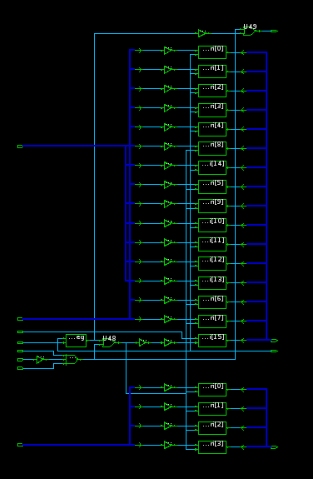
\includegraphics [scale = 0.8] {resource/dp_circ}
\caption{Draw pixel circuit}
\label{fig:dpcircuit}
\end{figure}

\newpage 

In figuur \ref{fig:dpcircuit} hierboven zijn duidelijk alle tri-state buffers te zien, zonder de flipflops erachter. Uiteindelijk is het circuit netjes gerout met een efficientie van 67,83\% en slechts 516 transistors. In overleg met Erwin is besloten het circuit deze vorm te geven. Drawpixel is namelijk een klein blok en goed te passen naast de grotere vierkante blokken op de chip in deze vorm. Dit zorgt wel voor meer transistoren, eerst was een efficientie van 85\% procent mogelijk. 
\begin{figure} [h!]
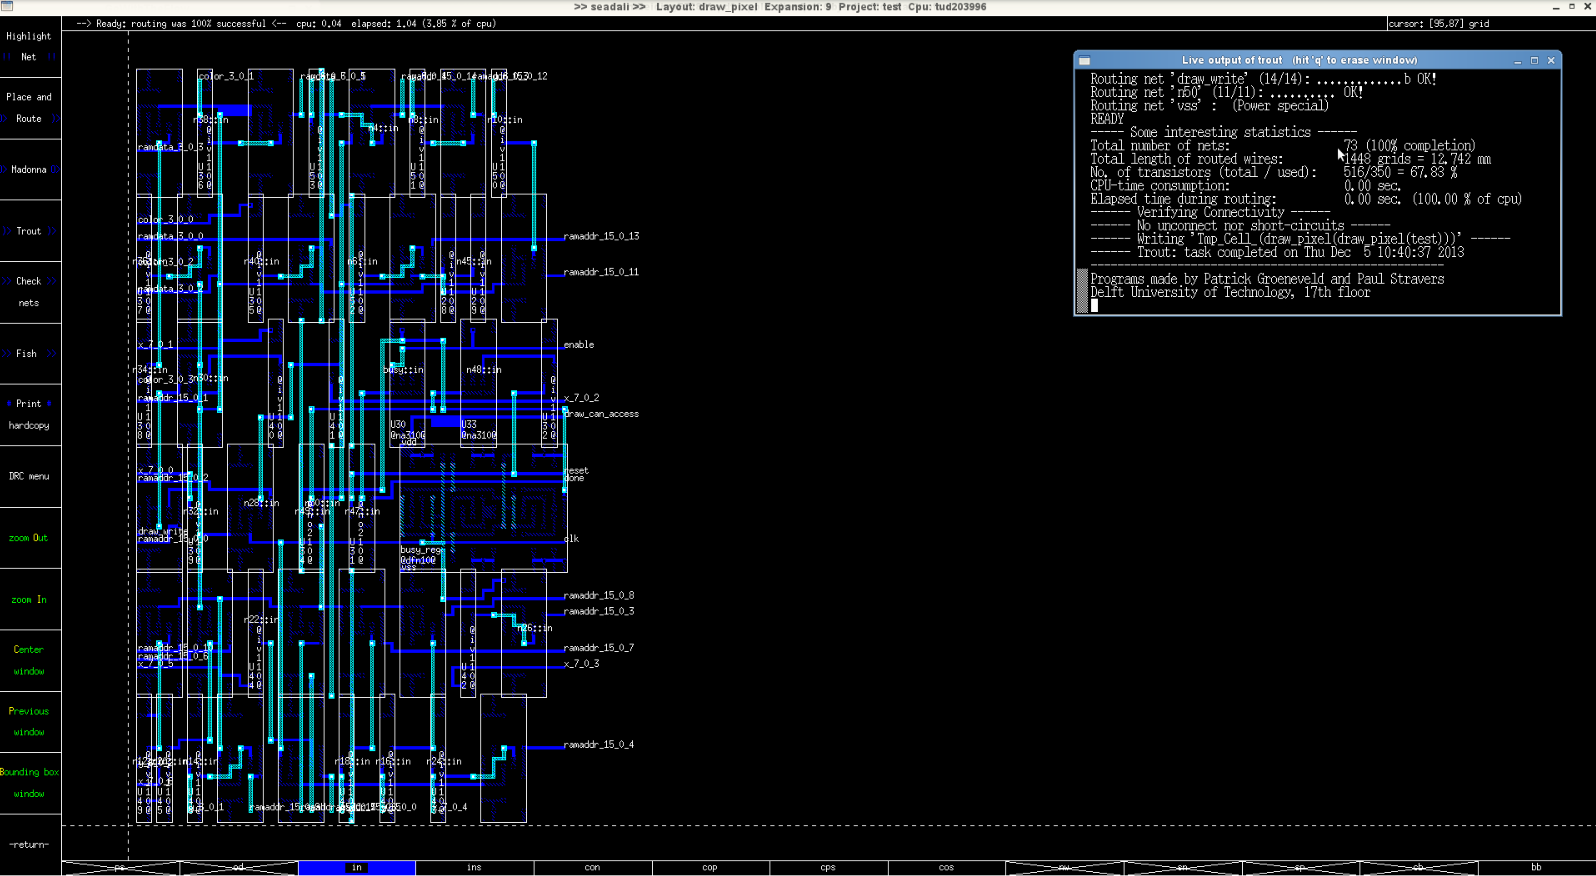
\includegraphics [width = \textwidth] {resource/dp_trout}
\caption{Synthesised en routed circuit}
\label{fig:dplayout}
\end{figure}

\subsection{Testplan en resultaten}
 De simulatie op transistor niveau komt goed overeen met de resultaten van de oorspronkelijke VHDL simulatie zoals in de afbeeldingen hieronder te zien is. Wanneer draw\_write naar '0' gaat, wordt done '1'  en ramaddr en ramdata 'Z'. Dat is volgens de specificaties. 
\begin{figure} [h!]
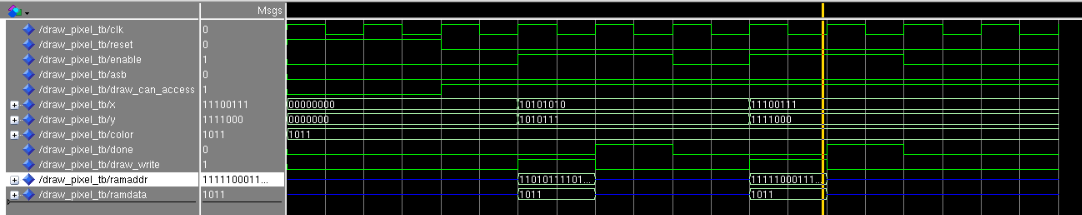
\includegraphics [width = \textwidth] {resource/dp_sim}
\caption{VHDL simulatie}
\label{fig:dp_sim}
\end{figure}

\begin{figure} [h!]
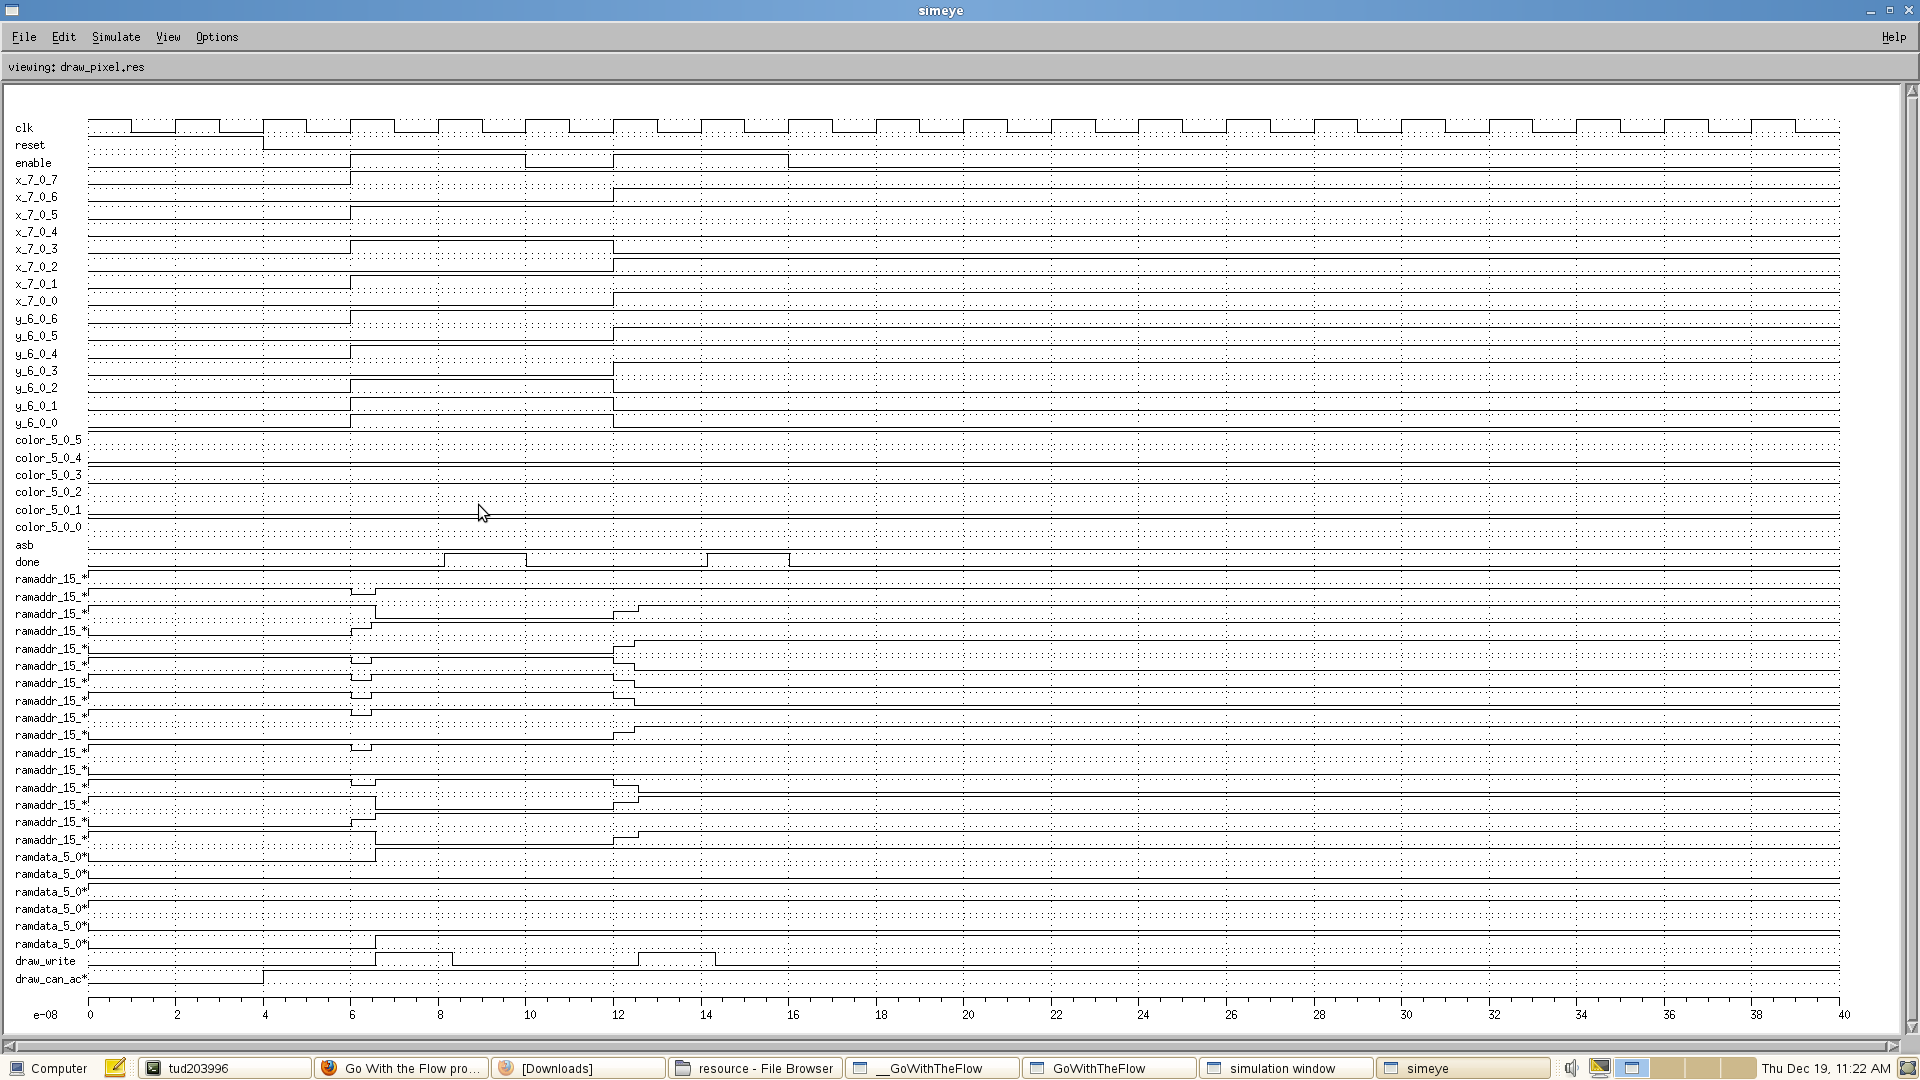
\includegraphics [width = \textwidth] {resource/dp_sw_lev}
\caption{Simulatie op transistor niveau}
\label{fig:dp_sw_lev}
\end{figure}
Uit de afbeeldingen \ref{fig:dp_sim} en \ref{fig:dp_sw_lev} valt te concluderen dat het blok werkt zoals het is ontworpen in VHDL. 1 klokslag nadat er een x, y en asb aan de ingangen wordt aangeboden, wordt er een stabiel ramadres aangeboden (klokslag 6-7). 1 klokslag daarna is done hoog. Omdat draw\_write 0 is geworden, gaat ramaddr als het goed is naar z
 Tot slot is er nog de mogelijkheid tot vergelijking van de simulaties binnen Go With The Flow, dat leidde tot de resultaten hieronder.
\begin{figure} [h!]
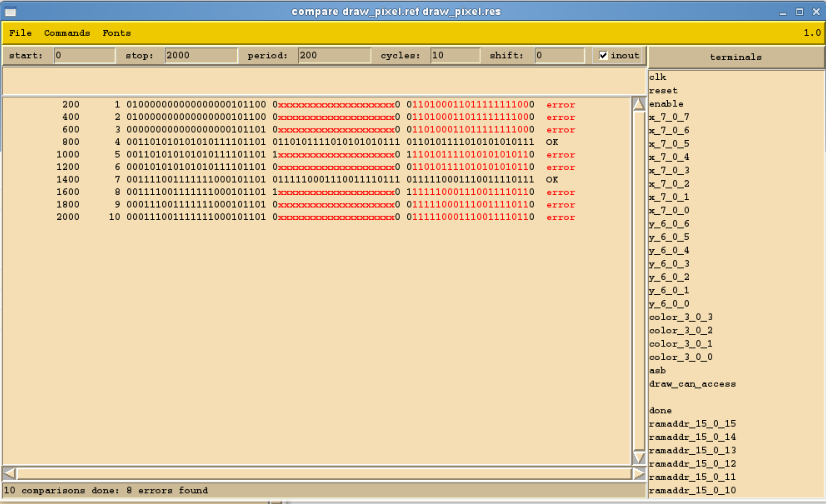
\includegraphics [width = \textwidth] {resource/dp_comp}
\caption{GWTF compare}
\label{fig:dp_comp}
\end{figure}
Het bovenstaande is correct, aangezien alle x niet worden begrepen omdat dat 'Z' is. Verder functioneert het ook helemaal zoals verwacht.

\subsection{Discussie}
Nadat de VHDL code als werkend kon worden beschouwd, moest de code worden gesynthetiseerd. In eerste instantie leverde dat 3000 transistoren op. Er is toen besloten de VHDL code op te delen in een sequentieel en een combinatorisch deel. Daarna is de code opnieuw gesynthetiseerd.  Echter na deze synthetisatie en ook wanneer er zelf blokken werden versleept kwamen we uit op 1500 transistors. Het grotere probleem was het feit dat hij hem moeilijk kon routen, maar na het circuit nader te bekijken zagen we dat er onnodig flipflops na da tri-state buffer kwamen, die vervolgens ook geen ‘Z’ konden opslaan. Dit zorgde voor de nodige errors, en een onnodig gebruik van extra flipflops. In de VHDL code hebben we vervolgens alle onnodige flipflops eruit gewerkt, waardoor alles in een keer werkte, en we dus ons uiteindelijke resultaat hebben behaald met slechts 516 transistors in plaats van 3000. 


\end{document}
